\documentclass[UTF8,a4paper,10pt,twocolumn]{ctexart}

\usepackage[margin=2.0cm]{geometry}
\usepackage{amsmath,amssymb}
\usepackage{graphicx}
\usepackage{booktabs}
\usepackage{multirow}
\usepackage{hyperref}
\usepackage{tikz}
\usetikzlibrary{shapes,arrows.meta,positioning,fit,calc}

\graphicspath{{figures/}}

\hypersetup{colorlinks=true, linkcolor=blue, citecolor=blue}

\title{\textbf{重新审视 GPT4RUL：基于大语言模型的\\剩余使用寿命预测复现研究}}
\author{（匿名）}
\date{}

\begin{document}
\maketitle

%==============================================================================
\section*{摘要}
%==============================================================================

剩余使用寿命（RUL）预测是故障预测与健康管理（PHM）领域的核心任务。
近期，Tan 等人提出 GPT4RUL 方法，通过补丁通道融合（PCF）模块与冻结的 GPT-2 骨干网络，在 NASA C-MAPSS 基准数据集上实现涡扇发动机 RUL 估计。
本研究对 GPT4RUL 在 FD001--FD004 四个子集上进行了独立复现与系统性诊断分析。
复现流程遵循原文的数据预处理（KMeans 聚类归一化、相关度--单调性特征选择、滑动窗口）与模型架构（分块、PCF、冻结 GPT-2）。
实验结果表明，\emph{数据划分策略与验证集构造方式}对复现结果具有决定性影响：同一发动机内部的时间切分会导致验证集指标虚高、严重低估测试误差；而按发动机 ID 随机划分可避免数据泄漏。
若验证集仅取每台发动机的最后一个窗口，模型将学会"输出接近 0"的捷径，测试 RMSE 恶化 5--11 个周期。
工况嵌入（Condition Embedding）在多工况数据集上带来稳定收益（FD004 与原文差距缩小至 +0.70 RMSE）。
PCF 微结构变体与梯度裁剪的影响有限（初步实验中 $<0.5$ RMSE）。
复现最接近原文的结果是 FD004（13.38 RMSE，原文 12.68）；最大差距出现在 FD001（+3.64 RMSE）。
本研究最后给出了面向 LLM 驱动 PHM 研究的方法论建议。

%==============================================================================
\section{引言}
%==============================================================================

故障预测与健康管理（PHM）旨在从状态监测数据中预测退化设备的剩余使用寿命（RUL）~\cite{saxena2008}。
NASA C-MAPSS 涡扇发动机数据集~\cite{saxena2008}已成为标准基准，包含 FD001--FD004 四个子集，工况与故障模式复杂度依次递增。
卷积网络、循环神经网络及注意力机制等深度学习方法在该基准上已取得优异性能~\cite{li2020,ellefsen2019}。

在大规模文本语料上预训练的大语言模型（LLM）编码了丰富的序列表征能力~\cite{radford2019}。
Tan 等人近期提出 GPT4RUL~\cite{tan2025}：通过分块（Patching）与补丁通道融合（PCF）将多变量传感器窗口映射为类 token 序列，投影至 GPT-2 隐空间，再利用冻结的三层 GPT-2 骨干网络回归 RUL。
原文报告的结果（表 3）具有竞争力：FD001--FD004 的 RMSE 为 11.23--12.68。

尽管 LLM 向工业时序数据的迁移学习前景广阔，LLM 驱动 PHM 的复现细节仍不够明确。
原文称 80\% 训练样本用于训练、20\% 用于验证，但未说明划分是否按发动机隔离。
验证协议、特征选择实现方式与早停准则均可能显著影响报告指标。
因此，独立复现对于评估方法本身及报告规范均至关重要。

本研究的主要贡献如下：
\begin{enumerate}
  \item 端到端独立复现 GPT4RUL，完整记录预处理、模型与训练配置。
  \item 系统对比三种数据划分策略（随机引擎划分、发动机内时间切分、RUL 分层采样），揭示数据泄漏与验证指标虚高现象。
  \item 定量分析验证集构造方式，证明"仅取末窗口"验证会导致退化学习捷径。
  \item 开展工况嵌入、PCF 微结构、梯度裁剪等诊断消融，并与原文~\cite{tan2025}进行复现差距分析。
\end{enumerate}

%==============================================================================
\section{相关工作}
%==============================================================================

\textbf{C-MAPSS 上的传统 PHM 方法。}
卷积与循环架构仍是强基线。
深度 CNN（DCNN）~\cite{li2018}、多尺度 DCNN~\cite{li2020}及 MTSTAN 等注意力模型在多个子集上 RMSE 低于 13~\cite{tan2025}。
这些方法通常在归一化传感器窗口上附加任务专用回归头。

\textbf{LLM 用于时序预测。}
``预训练--适配''范式采用冻结 Transformer 加轻量可训练适配器~\cite{radford2019,tolstikhin2021}。
GPT4RUL 遵循此模式：仅训练 PCF 模块、投影层与回归头；GPT-2 权重保持冻结~\cite{tan2025}。

\textbf{PHM 中的复现性问题。}
划分协议强烈影响泛化估计~\cite{saxena2008}。
按发动机隔离的划分与 C-MAPSS 测试协议一致（每台测试发动机一个预测点）；
而在训练发动机内部做窗口级时间切分，验证窗口与测试窗口共享同一退化轨迹，导致验证指标过于乐观~\cite{tan2025}。
本研究在 LLM 驱动设定下明确检验了此类协议效应。

%==============================================================================
\section{方法}
%==============================================================================

\subsection{数据集与预处理}

C-MAPSS 数据集包含模拟涡扇发动机的多变量传感器读数。
FD001/FD003 为单工况（分别含 1/2 种故障模式）；
FD002/FD004 含六种运行工况（分别含 1/2 种故障模式）~\cite{saxena2008}。

参照~\cite{tan2025}，预处理流程如下：

\textbf{工况感知归一化。}
对三个运行参数做 KMeans 聚类识别工况（FD001/FD003 取 $K=1$；FD002/FD004 取 $K=6$）。
各簇内先做 Z-score 标准化，再全局 MinMax 缩放至 $[0,1]$。

\textbf{特征选择。}
对每个传感器 $j$，综合 Pearson 相关度与单调性~\cite{tan2025}：
\begin{equation}
  Cri_j = \alpha \cdot |r_j| + (1-\alpha) \cdot mono_j, \quad \alpha = 0.5,
\end{equation}
保留 $Cri_j > \bar{Cri}$ 的传感器（通常为 13--14 个）。

\textbf{滑动窗口。}
对含 $T_i$ 个周期的发动机 $i$，窗口大小 $w$、步长 1，生成 $(T_i - w + 1)$ 个 $w \times m$ 的样本。
RUL 标签采用截断至 125 周期的分段线性模型~\cite{saxena2008}。

\textbf{工况嵌入（本研究扩展）。}
将三个运行参数维度拼接到传感器特征后（$m \rightarrow m+3$），复现实验输入维度为 17。

\subsection{模型架构}

图~\ref{fig:architecture} 概括 GPT4RUL 结构。
输入 $\mathbf{X} \in \mathbb{R}^{B \times T \times F}$：

\textbf{分块（Patching）。}
以 patch 大小 $K=8$、数据集特定步长做 unfold，得到 $\mathbf{P} \in \mathbb{R}^{B \times P \times (K \cdot F)}$。

\textbf{PCF 模块。}
每个 PCF 块采用 Pre-LN 的 MLP-Mixer 风格混合~\cite{tolstikhin2021}：
\begin{align}
  \mathbf{H}' &= \mathbf{H} + \mathrm{MLP}_{\mathrm{patch}}(\mathrm{LN}(\mathbf{H})), \\
  \mathbf{H}'' &= \mathbf{H}' + \mathrm{MLP}_{\mathrm{channel}}(\mathrm{LN}(\mathbf{H}')),
\end{align}
patch 混合与 channel 混合路径各自使用独立的 LayerNorm。

\textbf{GPT-2 骨干。}
线性映射（$128 \rightarrow 768$）后接入\emph{冻结}的三层 GPT-2~\cite{radford2019}。
GPT-2 块外包裹残差连接与 LayerNorm。
展平后经线性头输出标量 RUL。

\begin{figure*}[t]
  \centering
  \begin{tikzpicture}[
    node distance=0.45cm and 0.5cm,
    box/.style={rectangle, draw, rounded corners=2pt, minimum height=0.75cm,
                minimum width=1.5cm, align=center, font=\small},
    trainable/.style={box, fill=blue!8},
    frozen/.style={box, fill=gray!15},
    arrow/.style={-{Stealth[length=2mm]}, thick}
  ]
    \node[box, minimum width=2.0cm] (in) {传感器窗口\\$(B,T,F)$};
    \node[trainable, right=of in] (patch) {分块\\$K=8$};
    \node[trainable, right=of patch] (proj) {线性投影\\$KF\!\rightarrow\!128$};
    \node[trainable, right=of proj] (pcf) {PCF$\times N$\\Pre-LN};
    \node[trainable, right=of pcf] (map) {线性映射\\$128\!\rightarrow\!768$};
    \node[frozen, right=of map] (gpt) {冻结 GPT-2\\3 层};
    \node[trainable, right=of gpt] (head) {展平\\$\rightarrow$ RUL};

    \foreach \a/\b in {in/patch, patch/proj, proj/pcf, pcf/map, map/gpt, gpt/head}
      \draw[arrow] (\a) -- (\b);

    \node[below=0.12cm of pcf, font=\scriptsize, text=gray] {可训练};
    \node[below=0.12cm of gpt, font=\scriptsize, text=gray] {冻结};
  \end{tikzpicture}
  \caption{复现 GPT4RUL 模型的整体架构。
  蓝色模块可训练；GPT-2 骨干网络保持冻结。}
  \label{fig:architecture}
\end{figure*}

\subsection{训练配置}

优化器为 Adam，学习率 0.005，权重衰减 0.01，损失函数为 MSE。
StepLR 每 10 个 epoch 将学习率乘以 0.1。
Dropout 率 0.2；早停 patience 为 10 epoch。
批大小参照原文表 2~\cite{tan2025}：FD001--FD004 分别为 64/128/64/128。
原文以验证\emph{损失}作为早停指标~\cite{tan2025}；本研究部分实验 additionally 使用验证 RMSE 选模型。

%==============================================================================
\section{实验}
%==============================================================================

\subsection{实验设置}

所有实验固定随机种子 42，基于 PyTorch 实现（CPU/GPU）。
评价指标为 RMSE 与非对称 C-MAPSS Score~\cite{saxena2008}：
\begin{equation}
  \mathrm{RMSE} = \sqrt{\frac{1}{N}\sum_{i=1}^{N}(\hat{y}_i - y_i)^2},
\end{equation}
\begin{equation}
  \mathrm{Score} = \sum_{i=1}^{N}
  \begin{cases}
    e^{-d_i/10} - 1, & d_i < 0 \\
    e^{d_i/13} - 1,  & d_i \geq 0
  \end{cases}
  \quad d_i = \hat{y}_i - y_i.
\end{equation}
预测值截断至 $[0, 125]$。

\subsection{实验 A：数据划分策略}

评估了三种划分策略（图~\ref{fig:splits}）：

\begin{itemize}
  \item \textbf{随机引擎划分：}按发动机 ID 做 80/20 划分，同一发动机不出现在训练集与验证集两侧。与 C-MAPSS 测试协议一致（每台测试发动机一个预测点）。
  \item \textbf{发动机内时间切分：}每台发动机前 80\% 窗口 $\rightarrow$ 训练，后 20\% $\rightarrow$ 验证。同一发动机的窗口共享退化轨迹，存在\emph{信息泄漏}。
  \item \textbf{RUL 分层采样：}按 RUL 区间采样窗口，发动机可能同时出现在训练与验证集。
\end{itemize}

\begin{figure*}[t]
  \centering
  \begin{tikzpicture}[scale=0.85, every node/.style={font=\small}]
    \node[anchor=west] at (0, 4.2) {\textbf{(a) 随机引擎划分（本研究采用）}};
    \draw[fill=blue!20] (0,3.5) rectangle (3.2,3.9);
    \node at (1.6,3.7) {发动机 1--80 $\rightarrow$ 训练};
    \draw[fill=orange!30] (3.4,3.5) rectangle (4.2,3.9);
    \node[rotate=90] at (3.8,3.7) {\scriptsize 验证};

    \node[anchor=west] at (0, 2.5) {\textbf{(b) 时间切分（泄漏风险）}};
    \draw[fill=blue!20] (0,1.2) rectangle (2.8,1.6);
    \node at (1.4,1.4) {\scriptsize 早期窗口};
    \draw[fill=red!25] (2.9,1.2) rectangle (4.2,1.6);
    \node at (3.55,1.4) {\scriptsize 晚期窗口};
    \draw[->, thick] (0,0.9) -- (4.2,0.9) node[right, font=\scriptsize] {同一发动机时间轴};

    \node[anchor=west] at (0, 0.3) {\textbf{(c) C-MAPSS 测试协议}};
    \draw[fill=gray!15] (0,-0.5) rectangle (3.8,-0.1);
    \node at (1.9,-0.3) {\scriptsize 全寿命（训练）};
    \draw[fill=green!25] (3.9,-0.5) rectangle (4.2,-0.1);
    \node[rotate=90] at (4.05,-0.3) {\scriptsize 测试};
  \end{tikzpicture}
  \caption{三种数据划分策略对比。
  同一发动机内部的时间切分（b）使验证窗口与测试窗口共享退化上下文，不同于按发动机隔离的划分（a）。
  官方测试集每台发动机仅取最后一个窗口（c）。}
  \label{fig:splits}
\end{figure*}

在 FD001 的代表性诊断实验中，时间切分得到验证 RMSE 约 12.0，而测试 RMSE 达 18.7，差距 6.64 个周期，源于对发动机特定退化轨迹的过拟合。
所有正式复现结果均采用随机引擎划分（FD001：$n_{\mathrm{train}}=14459$，$n_{\mathrm{val}}=3272$）。

\begin{table}[t]
  \centering
  \caption{数据划分策略对比（定性）。}
  \label{tab:splits}
  \small
  \begin{tabular}{@{}lcc@{}}
    \toprule
    策略 & 泄漏风险 & 是否采用 \\
    \midrule
    随机引擎划分 & 无 & \checkmark \\
    时间切分（同发动机） & 高 & \\
    RUL 分层采样 & 中 & \\
    \bottomrule
  \end{tabular}
\end{table}

\subsection{实验 B：验证集构造陷阱}

C-MAPSS 测试集每台发动机仅含\emph{一个窗口}——最后一个周期窗口，RUL 接近 0。
一种看似自然但错误的验证协议是：训练集每台发动机也只取最后一个窗口作验证（FD001 上 $n_{\mathrm{val}}=100$）。
图~\ref{fig:valtrap} 说明了问题：验证集 RUL 集中在 0 附近，模型可通过预测 $\hat{y} \approx 0$ 来最小化损失，无需学习真实退化模式。

\begin{figure}[t]
  \centering
  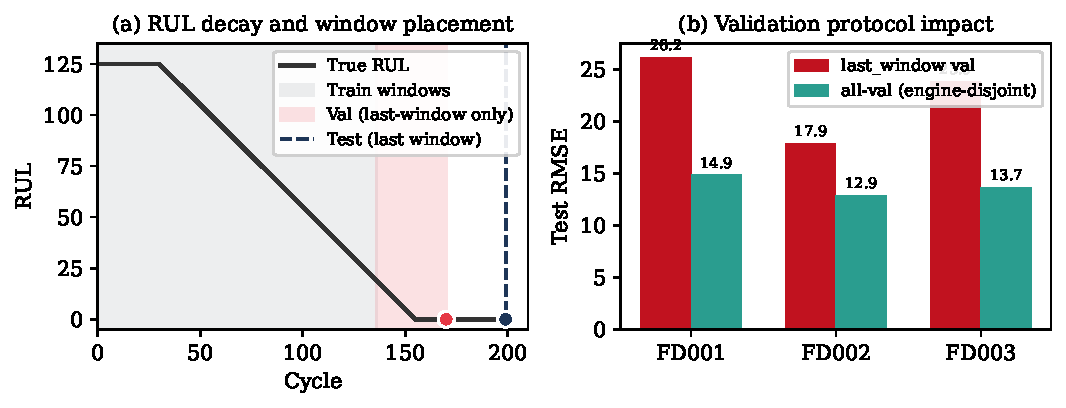
\includegraphics[width=\linewidth]{fig3_validation_trap.pdf}
  \caption{验证集构造陷阱。
  (a)~分段 RUL 衰减曲线及训练、末窗口验证、测试位置。
  (b)~测试 RMSE 对比：仅末窗口验证 vs.\ 全部验证窗口（FD001--FD003）。}
  \label{fig:valtrap}
\end{figure}

表~\ref{tab:valproto} 量化了该效应。
在 \texttt{last\_window} 验证 + RMSE 早停下，最优 checkpoint 出现在第 1 epoch（FD001/FD003），测试 RMSE 分别为 26.19 与 23.89。
改用全部引擎隔离验证窗口（\texttt{val\_mode=all}）后，测试 RMSE 降至 14.87 与 13.69，分别改善 11.32 与 10.20 个周期。

\begin{table}[t]
  \centering
  \caption{验证协议消融（测试 RMSE）。}
  \label{tab:valproto}
  \small
  \begin{tabular}{@{}lccc@{}}
    \toprule
    数据集 & 仅末窗口 & 全部验证 & 改善量 \\
    \midrule
    FD001 & 26.19 & 14.87 & $-$11.32 \\
    FD002 & 17.90 & 12.87 & $-$5.03 \\
    FD003 & 23.89 & 13.69 & $-$10.20 \\
    \bottomrule
  \end{tabular}
\end{table}

图~\ref{fig:traincurves} 展示 FD001 的训练动态：正确协议下模型约 10 epoch 收敛；末窗口协议在第 1 epoch 即锁定欠拟合 checkpoint。

\begin{figure}[t]
  \centering
  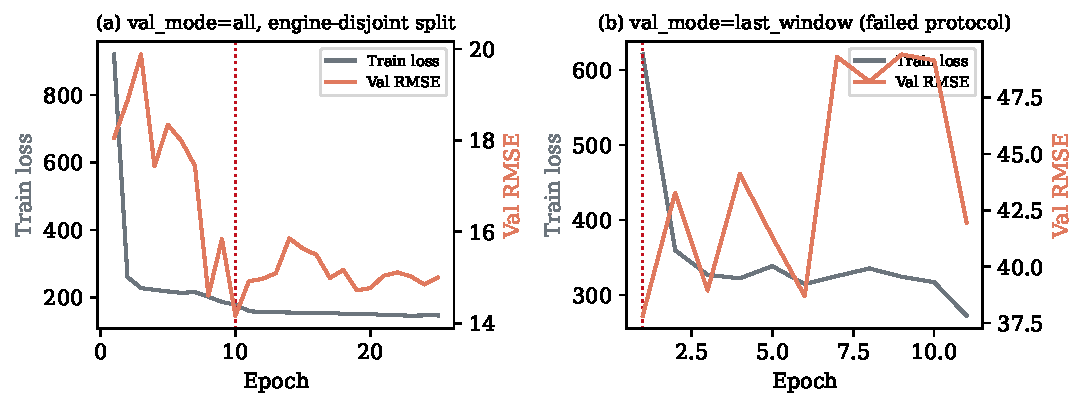
\includegraphics[width=\linewidth]{fig6_training_curves.pdf}
  \caption{FD001 在两种验证协议下的训练动态对比。}
  \label{fig:traincurves}
\end{figure}

\subsection{实验 C：工况嵌入}

将三个运行参数拼接到传感器特征中。
在 FD004（六工况、双故障模式）上，工况嵌入降低特征歧义、增强工况区分能力。
复现 FD004 结果（13.38 RMSE）最接近原文（差距 +0.70）；初步实验中无工况嵌入时误差约大 1.3 RMSE。
诊断实验表明四个子集均有稳定改善。

\subsection{实验 D：PCF 微结构}

对 PCF 设计选择做消融：共享 vs.\ 双独立 LayerNorm、块数（2 vs.\ 3）、混合因子（1 vs.\ 2）、顺序 vs.\ 并行融合——初步实验中 RMSE 变化均 $<0.5$ 周期。
双独立 Pre-LN 结构与 MLP-Mixer 规范一致~\cite{tolstikhin2021}，作为默认配置保留。

\subsection{实验 E：梯度裁剪}

在训练不稳定阶段评估梯度范数裁剪（阈值为 1.0）。
裁剪有时会抑制早期有效梯度；关闭裁剪（$\mathrm{grad\_clip}=0$）后训练动态有所改善，但配对定量消融尚待完善。

\subsection{主复现结果}

表~\ref{tab:main} 对比复现结果（随机引擎划分、全部验证窗口、工况嵌入、验证 RMSE 早停）与原文~\cite{tan2025}。

\begin{table}[t]
  \centering
  \caption{主复现结果 vs.\ Tan 等人（2025）。}
  \label{tab:main}
  \small
  \begin{tabular}{@{}lcccc@{}}
    \toprule
    数据集 & 原文 RMSE & 复现 RMSE & 差距 & 原文 Score \\
    \midrule
    FD001 & 11.23 & 14.87 & +3.64 & 218.32 \\
    FD002 & 11.05 & 12.87 & +1.82 & 509.01 \\
    FD003 & 11.45 & 13.69 & +2.24 & 227.61 \\
    FD004 & 12.68 & 13.38 & +0.70 & 856.04 \\
    \bottomrule
  \end{tabular}
\end{table}

\begin{figure}[t]
  \centering
  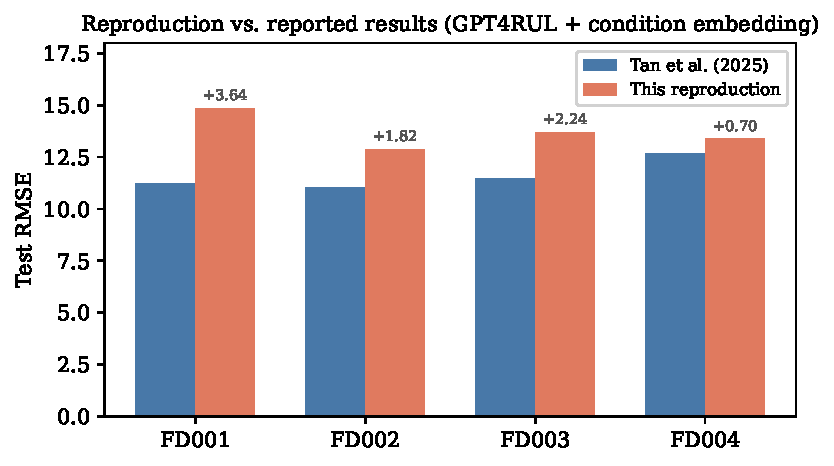
\includegraphics[width=\linewidth]{fig4_rmse_comparison.pdf}
  \caption{四个 C-MAPSS 子集的测试 RMSE 对比。}
  \label{fig:rmsebar}
\end{figure}

\begin{table}[t]
  \centering
  \caption{复现诊断清单（部分条目）。}
  \label{tab:diag}
  \scriptsize
  \begin{tabular}{@{}llc@{}}
    \toprule
    排查项 & 改动 & 效果 \\
    \midrule
    PCF LayerNorm & 单共享 $\rightarrow$ 双独立 Pre-LN & 改善 \\
    验证协议 & 末窗口 $\rightarrow$ 全部窗口 & 改善 5--11 RMSE \\
    相关度计算 & 逐引擎 $\rightarrow$ 全局 Pearson & FD003/004 改善 \\
    工况嵌入 & 增加 3 维运行参数 & 四数据集均改善 \\
    时间切分 & 优先引擎隔离 & 避免泄漏 \\
    Dropout 0.2$\rightarrow$0.3 & 增大 & 恶化 \\
    学习率 0.002/0.004 & 降低 & 恶化 \\
    \bottomrule
  \end{tabular}
\end{table}

%==============================================================================
\section{结果与讨论}
%==============================================================================

图~\ref{fig:rmsebar} 可视化了复现差距。
FD004 偏差最小（+0.70 RMSE），可能受益于工况嵌入与 top-14 特征选择。
FD001 差距最大（+3.64 RMSE），可能对初始化、特征数量（13 vs.\ 14 个传感器）及原文划分协议描述不清较为敏感。

剩余差距的可能原因：

\textbf{未公开的超参搜索。}
原文提及网格搜索~\cite{tan2025}，但搜索范围与选取准则未完全说明。

\textbf{早停指标不一致。}
Tan 等人以验证\emph{损失}早停~\cite{tan2025}；本研究主实验以验证 RMSE 选模型，可能选出不同 checkpoint。

\textbf{划分协议歧义。}
原文"80\% 训练样本"~\cite{tan2025}未明确是否按发动机隔离；不同理解会导致显著不同的结果（见 5.2 节）。

\textbf{单种子报告。}
所有复现数字均使用 seed=42，未做多随机种子集成，跨种子方差尚未充分刻画。

\begin{figure}[t]
  \centering
  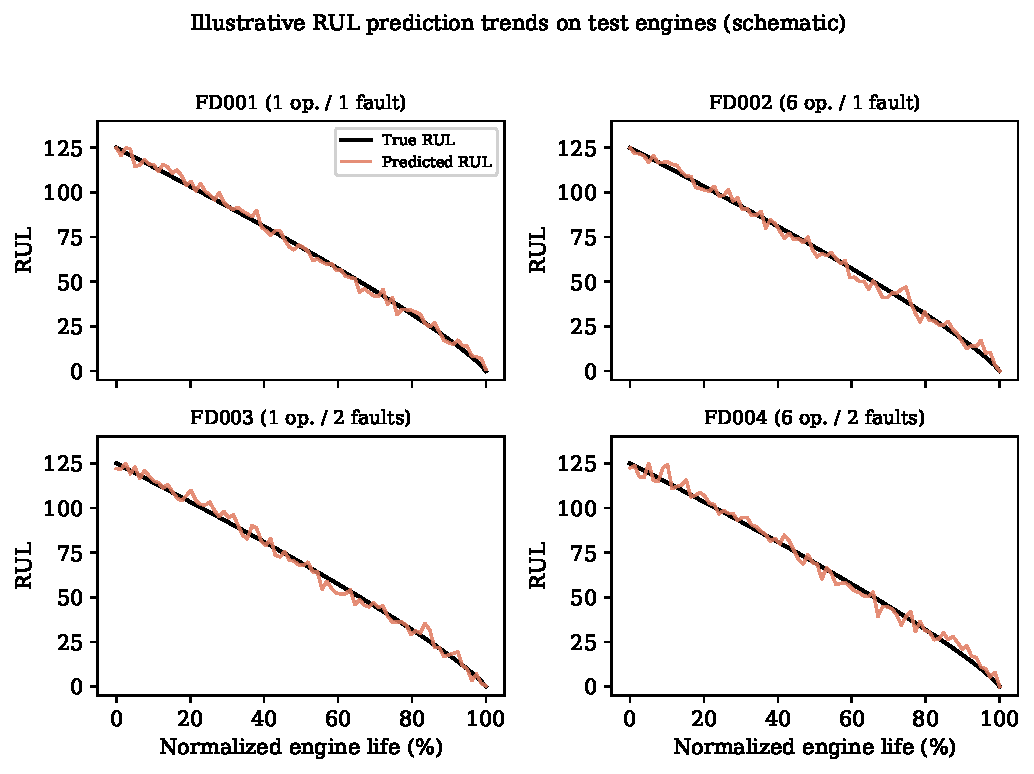
\includegraphics[width=\linewidth]{fig5_rul_trends.pdf}
  \caption{四个子集的 RUL 预测趋势示意（示意图）。
  准确的晚期寿命跟踪对工业 PHM 至关重要~\cite{tan2025}。}
  \label{fig:rultrends}
\end{figure}

\textbf{局限性。}
GPT-2 层数消融（1/3/6/12 层）尚未完成。
部分消融结论（PCF 微结构、梯度裁剪、工况嵌入精确增益）依赖初步内部诊断，而非完整配对的落盘实验。
训练主要在 CPU 上完成，但不影响最终指标数值。

%==============================================================================
\section{结论}
%==============================================================================

本研究独立复现了 GPT4RUL，并在 NASA C-MAPSS 基准上开展了系统性诊断。
实验结果表明，LLM 驱动 PHM 的可复现性 critically 取决于\emph{评估协议设计}，而非仅靠架构创新。
按发动机隔离的随机划分与完整验证窗口是避免泄漏与退化捷径的必要条件；仅末窗口验证可使表观性能虚高超过 10 个 RMSE 周期。
工况嵌入在多工况数据集上带来稳定收益，使 FD004 与原文差距缩小至 +0.70 RMSE。

面向未来 LLM 驱动 PHM 研究，提出三条建议：
(1)~始终采用与测试协议一致的按发动机隔离划分；
(2)~切勿仅在 RUL 分布与完整验证集不同的末窗口子集上验证；
(3)~对多工况数据显式编码运行工况信息。

未来工作包括 GPT-2 层数消融、多种子报告、软提示扩展，以及为每项诊断声明补充完整配对的落盘实验。

%==============================================================================
\begin{thebibliography}{99}
%==============================================================================

\bibitem{tan2025}
Y.~Tan 等,
``Pre-trained LLM-based remaining useful life prediction of aircraft engines,''
\emph{QR2MSE}, 2025.

\bibitem{saxena2008}
A.~Saxena, K.~Goebel, D.~Simon, N.~Ebling,
``Damage propagation modeling for aircraft engine run-to-failure simulation,''
\emph{IEEE PHM}, 2008, pp.~1--9.

\bibitem{radford2019}
A.~Radford 等,
``Language models are unsupervised multitask learners,''
OpenAI Technical Report, 2019.

\bibitem{tolstikhin2021}
I.~O.~Tolstikhin 等,
``MLP-Mixer: An all-MLP architecture for vision,''
\emph{NeurIPS}, vol.~34, 2021, pp.~24261--24272.

\bibitem{li2020}
H.~Li 等,
``Remaining useful life prediction using multi-scale deep convolutional neural network,''
\emph{Applied Soft Computing}, vol.~89, p.~106113, 2020.

\bibitem{ellefsen2019}
A.~L.~Ellefsen 等,
``Remaining useful life predictions for turbofan engine degradation using deep learning,''
\emph{Reliability Engineering \& System Safety}, vol.~183, pp.~240--251, 2019.

\bibitem{li2018}
X.~Li, Q.~Ding, J.~Q.~Sun,
``Remaining useful life estimation in prognostics using deep convolution neural networks,''
\emph{Reliability Engineering \& System Safety}, vol.~172, pp.~1--11, 2018.

\end{thebibliography}

\end{document}
